% DOCUMENT FORMATING
\documentclass[12pt]{article}
\usepackage[margin=1in]{geometry}

% PACKAGES
\usepackage{amsmath} % For extended formatting
\usepackage{amssymb} % For math symbols
\usepackage{amsthm} % For proof environment
\usepackage{array} % For tables
\usepackage{enumerate} % For lists
\usepackage{extramarks} % For headers and footers
\usepackage{fancyhdr} % For custom headers
\usepackage{graphicx} % For inserting images
\usepackage{multicol} % For multiple columns
\usepackage{verbatim} % For displaying code
\usepackage{tkz-euclide}
\usepackage{pgfplots}
\usepackage{gensymb}
\usepackage{mathtools}
\usepackage{graphicx}
% SET UP HEADER AND FOOTER


\title{MATH 242 - WS1}
\date{01/11/2024}


\begin{document}
\maketitle


\begin{enumerate}

\item Below is the graph of a function $f(x)$. Answer the following questions:

\begin{center}
    \includegraphics[scale=.45]{inverse.png} 
\end{center}

\begin{enumerate}
\item Is the function 1-to-1? How can you visually tell?
\vfill

\item Graph $f^{-1}(x)$ on the same $xy$-plane.
\vfill

\item  What is the domain of $f^{-1}$?
\vfill

\item What is the range or co-domain of $f^{-1}$?
\vfill

\item What is $f^{-1}(0)$?
\vfill
\end{enumerate}

\pagebreak

\item Let $f(x) = \dfrac{3}{1-x}$. Find $f^{-1}(x)$.

\vfill

\item Verify your answer from the previous problem by checking that $f^{-1}(f(x)) = x$.
\vfill
%\item  Let $f(x) = \dfrac{x+2}{1-x}$. Find $f^{-1}(x)$.

%\vfill

\item  Let $f(x) = \sqrt[3]{5-2x}$. Find $f^{-1}(x)$.

\vfill

\pagebreak



\item Find the domain and range of $f(x) = \dfrac{1-x}{x+2}$.  
\vfill


\item Consider this graph of $y=f(x)$ and answer the questions below:

\begin{center}
\includegraphics[scale=.4]{inverse2.png}
\end{center}

\begin{enumerate}

\item What is $f^{-1}(-4)$?
\item What is $f^{-1}(-2)$?
\item What is $f^{-1}(5)$?

\end{enumerate}

\vfill


\pagebreak

\item Show the given functions are indeed inverses functions (i) analytically (by calculating $(f\circ g)(x)$ or $(g\circ f)(x)$) and (ii) graphically.
$$f(x)=\frac{3x+4}{5}\quad\text{and}\quad g(x)=\frac{5x-4}{3}$$

\vfill
\begin{center}
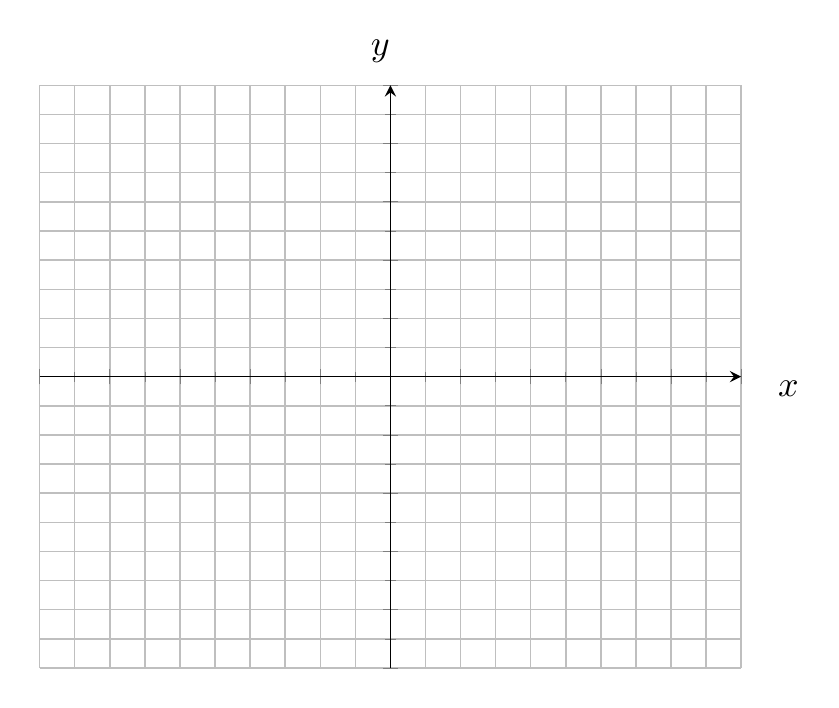
\begin{tikzpicture}[scale=1.3]
\begin{axis}[grid=both,ymin=-10,ymax=10,xmax=10,xmin=-10, xtick={-10,-8,-6,-4,-2,0,2,4,6,8,10}, 
ytick= {-10,-8,-6,-4,-2,0,2,4,6,8,10},
xticklabel=\empty,yticklabel=\empty,
minor tick num=1,axis lines = middle,xlabel=$x$,ylabel=$y$,label style =
{at={(ticklabel cs:1.1)}}]
\end{axis}
\end{tikzpicture}
\end{center}

\item Show the given functions are indeed inverses functions (i) analytically (by calculating $(f\circ g)(x)$ or $(g\circ f)(x)$) and (ii) graphically.
$$f(x)=2x^2+3\text{ for }x\in[0,\infty)\quad\text{and}\quad g(x)=\sqrt{\frac{x-3}{2}}$$

\vfill
\begin{center}
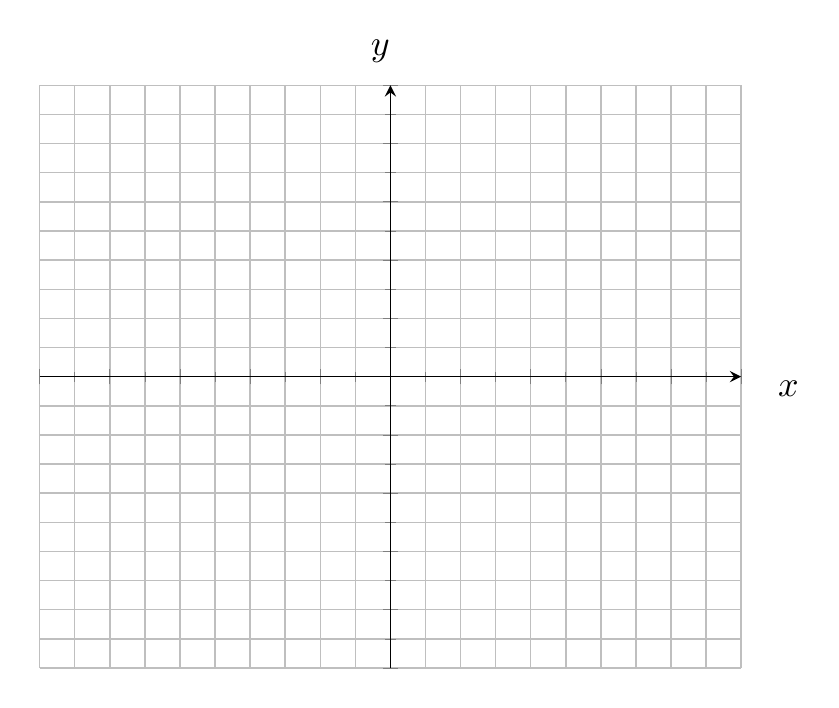
\begin{tikzpicture}[scale=1.3]
\begin{axis}[grid=both,ymin=-10,ymax=10,xmax=10,xmin=-10, xtick={-10,-8,-6,-4,-2,0,2,4,6,8,10}, 
ytick= {-10,-8,-6,-4,-2,0,2,4,6,8,10},
xticklabel=\empty,yticklabel=\empty,
minor tick num=1,axis lines = middle,xlabel=$x$,ylabel=$y$,label style =
{at={(ticklabel cs:1.1)}}]
\end{axis}
\end{tikzpicture}
\end{center}


\end{enumerate}
\end{document}
